\documentclass[a4paper]{article}
\usepackage[utf8]{inputenc}
\usepackage{textcomp}
\usepackage{geometry}
\geometry{ left=2cm, right=2cm, top=2cm, bottom=2cm, bindingoffset=5mm}
\usepackage{graphicx}
\usepackage{xcolor}
\usepackage{hyperref}
\date{}
\author{}
\usepackage{fancyhdr}
\pagestyle{fancy}
\fancyhf{}
\fancyhead[R]{2973140 - Felix Bühler \\ 2892258 - Gerhard Breul \\  3141241 - Jamie Ullerich}
\fancyhead[L]{Information Visualisation and Visual Analytics \\ WS 2019/20 }
\renewcommand{\headrulewidth}{0.5pt}
\usepackage{tikz}
\usetikzlibrary{calc}
\usepackage{amsmath}
\usepackage{cleveref}
\usepackage{subcaption}

\usepackage{changepage,lipsum,titlesec}
\titleformat{\section}[block]{\bfseries}{\thesection.}{1em}{}
\titleformat{\subsection}[block]{}{\thesubsection}{1em}{}
\titleformat{\subsubsection}[block]{}{\thesubsubsection}{1em}{}
\titlespacing*{\subsection} {2em}{3.25ex plus 1ex minus .2ex}{1.5ex plus .2ex}
\titlespacing*{\subsubsection} {3em}{3.25ex plus 1ex minus .2ex}{1.5ex plus .2ex}


\title{\textbf{Assignment 8}}

\begin{document}
\maketitle 
\thispagestyle{fancy}


\fbox{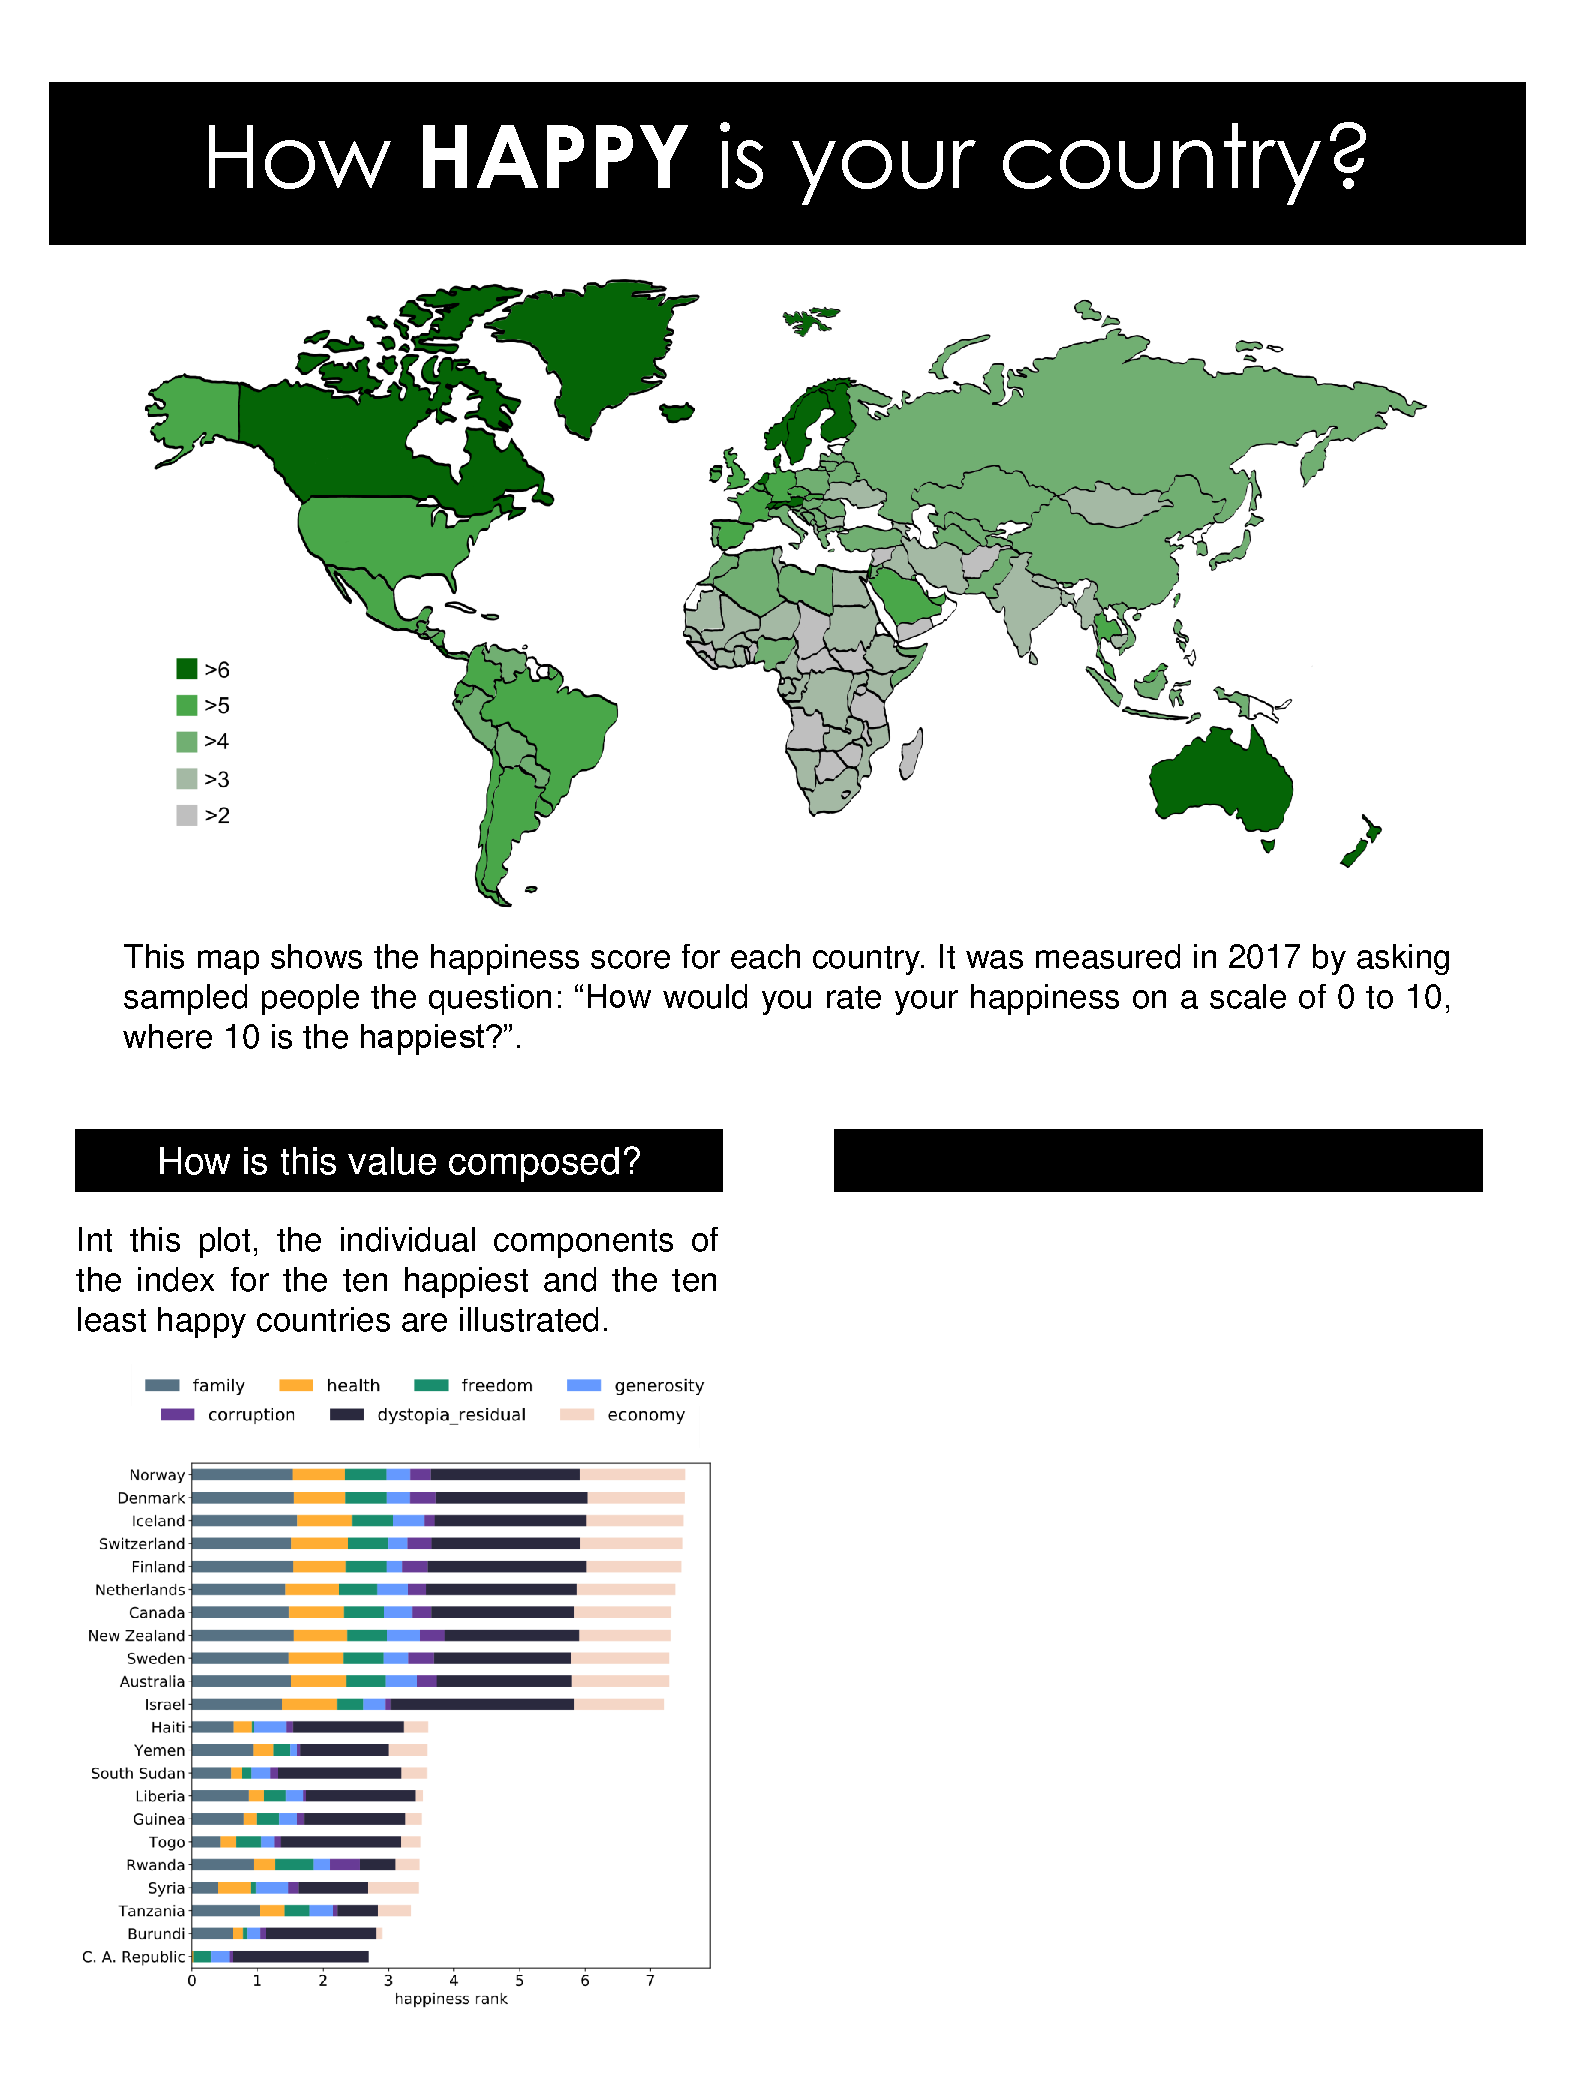
\includegraphics[width=0.98\linewidth]{HappyPoster.pdf}} \\

\section*{Task 1 - The happiness index by country}
\subsection*{(a) Visualizing the data}
%In either case, reflect and report in 3-10 sentences on the message of your poster/dashboard: if it is a storytelling assignment, what is the point of view you are conveying? if it is a data exploration assignment, what are potential conclusions an external viewer of your visualization might reach upon inspecting/reading your poster?
Our poster consists of three parts: first of all, there is a map at the top which shows the happiness score for each country on a map. 
This is supposed to give a quick overview on how the happiness is distributed across the world. 
Of course, this does not show any detail on the exact scores, therefore we created the more detailed visualisations at the bottom. 
The viewer could potentially see, that people in Africa seem to bee not as happy as in America or Europe.  
At the lower left corner, there is a bar chart which shows the ten happiest and least happy country. 
The ranking can be easily seen, as well as the difference between each country. 
Besides that, it shows the composition, which is also interesting, because it is possible to compare if one of the influencing factors is less or more present in happy or rather sad countries. 
Here, the relation between the grey areas in the map above and for example the health component can be see. 
A potential viewer might conclude, that there is for example less health and freedom in less happy countries which are mostly in Africa. 
So, these two visualisations cover the happiness score and how it is composed in detail. 
The third visualisation at the bottom right corner covers a different topic. 
It shows, that even if the freedom in this country is high, the internet access must be high as well to result in a high happiness. 
Since scatter plots might not be as easy to understand as the map or bar chart, there is a bit more text description to help viewer understand what is illustrated here. \\ \linebreak
% Briefly report on weaknesses and strengths of your visualization, as well as potential improvements.
One strength of this visualisation is the map. 
It is easy to understand and interesting for all kinds of people, even those wo do not like to interpret charts. 
One disadvantage is, like mentioned above, that it is not very accurate or detailed. 
But, we tried to cover the detail aspect with the lower plots. 
The advantage of the left plot is, that it shows a lot of details in one bar, without being to overwhelming. 
People who are not interested in the exact components can still see the ranking and difference between the countries. 
It might be interesting to see more countries, but at the same time this would be overwhelming since 150 countries are a lot. 
Instead of showing the top and last 10 countries it might would have been interesting to see the top 20, or some countries in the middle. 
The right plot shows the least info. 
There are only 3 different variables, but this avoids visual clutter and being to overwhelmed by information. 
It would have been possible to show much more information since the dataset contains a lot more useful data, but we decided to only illustrate interesting data without overwhelming the viewer. 
Additionally, it would have been possible to display the correlation between more than two columns like in the lower right plot, like in a scatter plot matrix for example, but we were not sure how easy people can understand this without spending to much time in front of the poster. 
The goal of our poster is therefore to give a quick overview with additional details, but showing more details would also be great when people are willed to spend more time to understand the poster. 


\subsection*{(b) Evaluation}
\subsection*{(c) Bonus Points}

\end{document}
